\chapter{Analyse de Levee}
\label{chap:levee}

% introduction du projet Levee... composant, équipe, epfl

\gls{levee} est un projet mené dans le cadre du Dependable Systems Lab \cite{dslab} par les chercheurs Volodymyr Kuznetsov, Laszlo Szekeres, Mathias Payer, George Candea, R. Sekar et Dawn Song. Le but annoncé du projet est de sécuriser tout programme informatique contre la totalité des attaques de type \og control-flow hijack \fg via une erreur mémoire, du moment où celui-ci a été compilé grâce à \gls{clang} avec les options nécessaires.

Comme montré dans le chapitre précédent, il existe déjà plusieurs mécanismes (\gls{dep}, \gls{aslr}) permettant de réduire le risque de ce type d'attaque sans imposer au programme de coût supplémentaire en matière de performance. Cependant, il est aujourd'hui possible de les contourner, même au sein d'un environnement de production, grâce à des attaques évoluées telles que le \gls{rop}. D'autres mécanismes plus évolués (\gls{cfi}, SoftBound+CETS, CCured ou encore AddressSanitizer) permettent quant à eux d'améliorer trés fortement la sécurité, mais ne permettent pas, soit de garantir une totale intégrité et reste à ce jour contournable, soit ils ne sont pas adoptés à grande échelle à cause de leurs effets beaucoup trop négatifs sur la performance du programme --- jusqu'à 116\% de coût en performance ---.

Le défi relevé par l'équipe de recherche a été de proposer un modèle de sécurité entrainant des coûts faibles en matière de performance tout en garantissant l'intégrité complète du flot de contrôle. \gls{levee} est le prototype d'implémentation de ce modèle et ce chapitre se concentre sur ses aspects théoriques, son implémentation au sein des outils de compilation \gls{llvm} et son rayon d'action.

\minitoc

\newpage

% -----------------------------------------------------------------------------
\section{Concepts théoriques}

Seules les attaques visant à dérouter le flot de contrôle de l'application sont prises en compte dans le modèle de sécurité. Les attaques du types \og data-only \fg, visant à modifier ou récupérer des informations qui ne font pas partie du flot, n'entrent pas en considération.

Ils émettent l'hypothèse que l'attaquant a le contrôle total sur la mémoire du processus et que le chargement du programme ainsi que le binaire ne peuvent pas être altérés. De ce fait, les mécanismes de protection résultant de la compilation peuvent se mettre en place avant l'intervention de l'attaquant.

Les chercheurs du projet posent comme postulat de départ qu'il est suffisant de garantir l'intégrité des pointeurs pour rendre impossible la modification du flot de contrôle via exploitation d'erreurs mémoires. Dans le cas des langages de types \og memory-safe \fg, un objet en mémoire ne peut être accédé que depuis un pointeur prévu explicitement pour l'objet en question. Cela rend la modification du flot de contrôle impossible, mais entraîne une baisse de performances importante.

Afin de garder de bonnes performances tout en garantissant l'intégrité complète, le minimum d'instrumentation doit être délégué à l'exécution. Le code est alors en premier lieu analysé de manière statique à la compilation, puis des mécanismes de vérification sont ensuite délégués à l'exécution. Le concept de \og \gls{cpi} \fg \cite{CPIPaper} intervient alors, afin de déterminer quels pointeurs doivent être protégés, ce qui permet de réduire au minimum les accès à controler lors de l'exécution.

\section{CPI (Code-pointer integrity)}

% Decrire pourquoi les pointeurs sensibles et pas sensibles. comment determiner si un pointeur est sensible

\subsection{Définition d'un \og code-pointer \fg}

Afin de formaliser les pointeurs de code (code-pointers), le papier propose la définition suivante :

On dit que l'indirection ou le déréférencement d'un pointeur est sûr si et seulement si l'adresse mémoire à laquelle il tente d'accéder est comprise au sein de l'\textit{objet mémoire} sur lequel le pointeur est \textit{basé}. Un \textit{objet mémoire} est une abstraction liée au langage définissant tout types de structures stockées en mémoire (variables globales, variables locales, structures, objets), de sous-structures (un champ d'une structure) ou encore des points de contrôle du flot (adresse de départ d'une fonction, adresse de retour). Ces \textit{objets mémoires} ont un cycle de vie défini, lorsqu'on libére la mémoire liée à un tableau et qu'on alloue un nouveau tableau avec la même adresse, un nouvel \textit{objet mémoire} est créé.

Le papier formalise ensuite la définition de pointeur \textit{basé sur} un \textit{objet mémoire}. On dit qu'un pointeur est \textit{basé sur} sur un \textit{objet mémoire X} si et seulement si le pointeur est obtenu lors de l'exécution par (i) allocation de \textit{X} sur la pile, (ii) référencement explicit de l'adresse de \textit{X}, (iii) en référencant l'adresse d'un sous-objet \textit{y} de \textit{X} (accès au champ \textit{y} d'une structure \textit{X}), ou (iv) en effectuant une expression sur un pointeur (calculs arithmétiques, position au sein d'un tableau, copie de pointeur) impliquant l'adresse de l'\textit{objet mémoire X}. Cette définition est basée sur la définition des pointeurs \textit{basé sur} présente au sein de la norme C99.

\newpage

Si l'on part maintenant du principe que ces deux définitions sont strictement respectées pour tout pointeurs, peu importe les paramètres donnés à l'exécution du programme, alors on peut qualifier le-dit programme de \textit{memory-safe}. Dans ce cas il n'est plus possible de dérouter le flot de contrôle en exploitant une erreur basée sur la mémoire.

\subsection{Concept théorique}

Le mécanisme de \gls{cpi} est statisfait si toutes les indirections ou les déréférencements sur les pointeurs accédant ou déréférençant des pointeurs jugés \og sensibles \fg sont sûrs. La définition des pointeurs jugés sensibles est donc récursive. Les pointeurs de départ devant être protégés sont les pointeurs responsables de transférer le flot de contrôle de l'application. Cette notion de récursivité est donc dynamique, un pointeur de type \mintinline{c}{void*} doit être considéré comme sensible s'il pointe vers une fonction ou sur un autre pointeur jugé sensible, mais ne doit pas être considéré comme sensible s'il pointe vers un type \mintinline{c}{int}.

Les langages de programmation bénéficiant d'une mémoire supervisée satisfont le concept de \gls{cpi}. Cependant, ils ne différencient pas les pointeurs sensibles des autres, ce qui entraîne une forte baisse de performance par rapport aux langages de type C/C++ (le papier mentionne une perte de $\geq2\times$ au sein des meilleures implémentations actuelles).

L'observation faite par l'équipe de chercheurs est la suivante: afin de garantir le flot de contrôle de l'application, seul l'accès aux pointeurs jugés sensibles doit être vérifié et ces pointeurs forment un ensemble de petite taille sur l'ensemble des pointeurs. Les pointeurs agissant sur les données peuvent se permettre de ne pas être controlés, ce qui augmente l'efficacité tout en maintenant un très haut taux de protection.

\subsection{Déterminer l'ensemble des pointeurs sensibles}

Afin de déterminer l'ensemble des pointeurs devant être considérés comme sensibles, une analyse statique est effectuée. Pour ce faire une heuristique simple est utilisée: \og un pointeur est jugé sensible si son type est sensible \fg. Les types marqués comme étant sensibles sont:

\begin{enumerate}
	\item pointeurs de fonction
	\item pointeurs vers des pointeurs sensibles
	\item pointeurs vers des types composés (\mintinline{c}{array}, \mintinline{c}{struct}) qui contiennent un ou plusieurs pointeurs sensibles
	\item pointeurs universels (\mintinline{c}{void*}, \mintinline{c}{char*})
  \item pointeurs explicitements créés par le compilateur ou à l'exécution (adresse de retour, tables virtuelles en C++ \cite{fonctionsVirtuelles}, \mintinline{c}{setjmp} \cite{setjmp})
\end{enumerate}

Cet ensemble de types peut être adapté, étendu, suivant les besoins du programme ou de la plateforme. Le papier mentionne en exemple la structure \mintinline{c}{ucred} utilisée dans le noyau FreeBSD, qui est marquée comme sensible car elle contient les UIDs des processus et d'autres informations.

En effectuant des tests, les chercheurs se sont rendu compte que l'analyse heuristique mettait en avant un ensemble de pointeurs correspondant en moyenne à $6.5\%$ de l'ensemble global. Ce chiffre met en avant l'impact sur l'efficacité qu'a cette approche.

Le coût en performance dépend directement de l'heuristique et de sa récursion. L'équipe mentionne elle-même que toutes heuristiques donnant un ensemble approximatif cohérent peuvent être utilisées. Des améliorations peuvent encore être attendues sur ce point. Le second avantage majeur de cette approche réside dans le fait que l'on peut facilement imaginer de nouvelles heuristiques permettant de protéger d'autres ensembles de pointeurs, par exemple, pour protéger une partie des données au sein du programme.

\subsection{Zone de mémoire sûre \og safe region \fg}

Afin de garantir l'intégrité de l'ensemble des pointeurs sensibles, une zone mémoire appelée \og \textit{safe region} \fg est créée, voir la \autoref{fig:safeRegionLayout}. Cette région est isolée et ne peut être accédée que via des instructions fournies par \gls{cpi}. Cela permet de garantir l'intégrité des données et la propagation des métadonnées. Elle est ensuite constituée d'un \og \textit{safe pointer store} \fg, pour les pointeurs sensibles, et de \og \textit{safe stacks} \fg, pour une gestion plus spécifique liée à la pile d'exécution, voir la \autoref{section:safeStack}. Seule l'une des deux copies présente dans les deux régions est utilisée suivant le type du pointeur en question.

\begin{figure}[H]
	\centering
	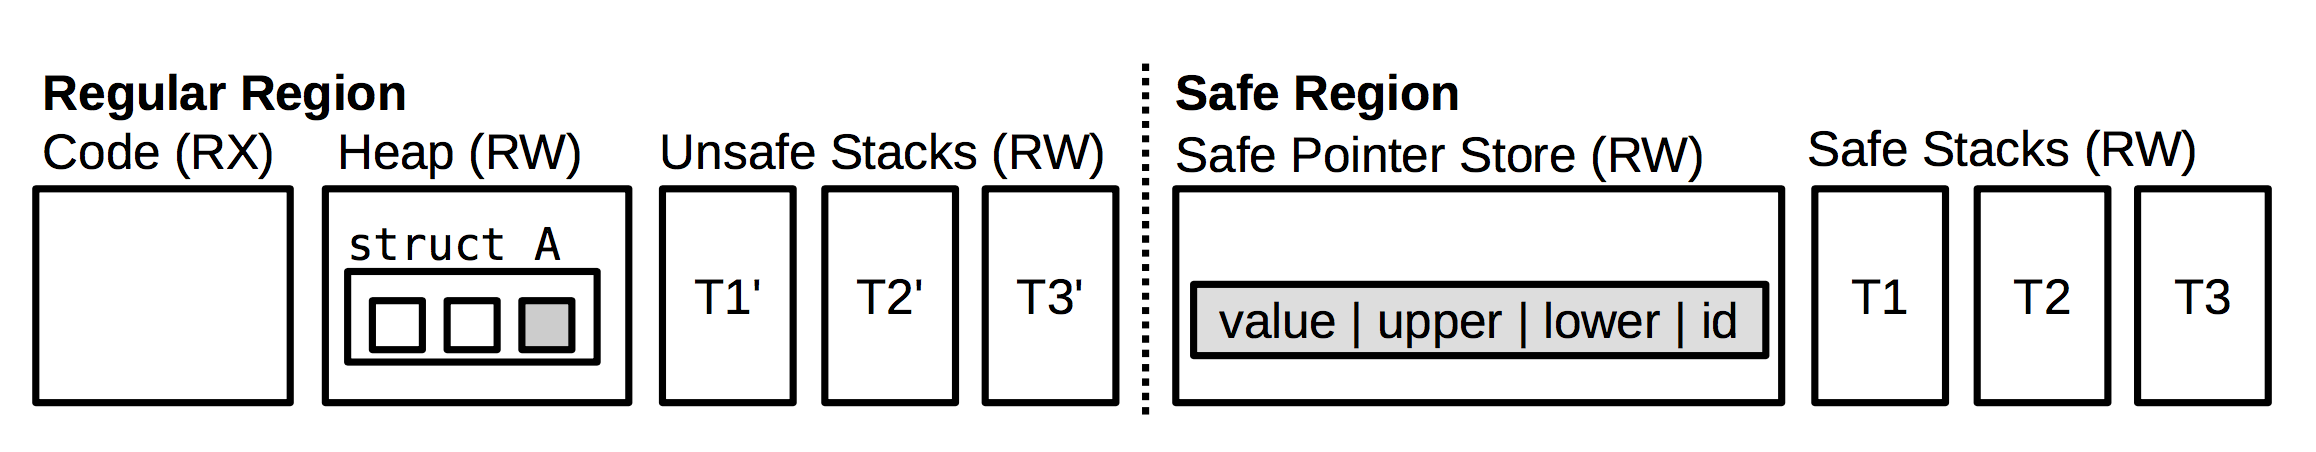
\includegraphics[width=1\columnwidth]{safeRegionLayout}
	\captionsource{Agencement de la mémoire avec CPI}
	{Agencement de la mémoire avec CPI, tiré du papier Code-Pointer Integrity}
	{\url{http://dslab.epfl.ch/pubs/cpi.pdf}}
	\label{fig:safeRegionLayout}
\end{figure}

Le \textit{safe pointer store} permet de stocker la valeur du pointeur et les métadonnées de l'\textit{objet mémoire} sur lequel le pointeur est \textit{basé}. Les métadonnées sont constituées de l'adresse de départ et de fin de l'objet au sein de la mémoire standard ainsi que d'un identifiant temporaire de l'objet en question. L'approche est similaire à celle utilisée au sein de SoftBounds+CETS \cite{SoftBound} à la différence prêt que \gls{cpi} stocke également la valeur du pointeur et n'applique pas de protection sur tout les pointeurs du programme.

\gls{cpi} garantit (i) que tous les pointeurs sensibles sont stockés dans la \og \textit{safe region} \fg, (ii) que la création et la modification lors de l'exécution de pointeurs sensibles soit propagée et (iii) que toutes les indirections ou les déréférences soient vérifiées grâce au métadonnées. Afin d'y parvenir, \gls{cpi}, lors de la phase de compilation, réécrit les instructions de création et d'accès de l'ensemble des pointeurs sensibles.

% on stocke l'adresse du pointeur dans la région standard ainsi que ca valeur = deux adresses
% TODO figure montrant qu'est ce qui est stocké et les liens

\subsection{Isolation de la zone de mémoire sûre}

Une fois les metadonnées et les \og \textit{safe stacks} \fg placées au sein de la région sûre, il faut pouvoir garantir leur intégrité. Pour ce faire cette région doit être isolée du reste de la mémoire et il ne doit pas être possible de la modifier sans passer par les instructions fournies par \gls{cpi}. Ce mécanisme de protection est directement dépendant de l'architecture pour laquelle le binaire est compilé. Dans les deux cas, la région sûre est placée dans le segment de \og memory mapping \fg avec un accès en lecture et écriture.

\subsubsection{Architecture 32~bits}

Dans le cas d'une architecture \texttt{x86-32}, la \og \textit{safe region} \fg est isolée grâce à l'utilisation des segments mémoires. Un segment mémoire n'étant pas utilisé au sein du programme est utilisé par \gls{cpi} afin de stocker l'adresse de base de la \og \textit{safe region} \fg. Les autres segments sont configurés afin de rendre l'accès à la région sûre impossible.

% \textit{TODO définition des segments, exemple d'utilisation etc... tout la sécu se base la dessus. Sinon ca revient à de l'ASLR}

La preuve de sécurité sous cette architecture repose sur le fait qu'il n'est pas possible, lors de l'exécution, d'atteindre ou de modifier le segment qui contient la région de mémoire sûre.

\subsubsection{Architecture 64~bits}

Au sein d'une architecture \texttt{x86-64} la limitation des segments n'est plus présente, mais l'architecture met toujours à disposition deux registres de segments mémoire. \gls{cpi} utilise l'un des deux segments pour stocker l'adresse mémoire de base pour la \og \textit{safe region} \fg. Cette adresse de base est tirée aléatoirement lors du lancement de l'application, ce qui ressemble fortement à l'approche d'\gls{aslr} expliquée en \autoref{section:aslr}. Cependant, la différence mentionée dans le papier est qu'il n'existe aucun pointeur vers la \og \textit{safe region} \fg au sein de la région standard, ce qui fait qu'il n'est pas possible de remonter jusqu'à l'adresse de base. Les 48~bits d'adressage offrent donc une sécurité suffisante et rendent impraticable une attaque par recherche exhaustive.

La preuve de sécurité, sous architecture \texttt{x86-64}, est donc basée sur des informations cachées. Ils mentionnent le fait que leur modèle est \og leak-proof \fg \ --- c’est-à-dire qu'il ne laisse pas fuiter d'informations concernant la localisation de la région sûre ---, à la différence d'\gls{aslr}, grâce à l'absence de pointeur vers la \og \textit{safe region} \fg lors de l'execution.


\section{CPS (Code-pointer separation)}

% Decrire la variante CPS, moins d'overhead mais permettant certain hijack

Les chercheurs se sont rendus compte que dans le cas du \texttt{C++}, l'ensemble des pointeurs sensibles peut rapidement devenir trop important pour cause, par exemple, d'utilisation de fonctions virtuelles. Tous les pointeurs vers un objet contenant une fonction viruelle deviennent alors sensibles, ce qui peut induire un coût de performance trop élevé. Pour palier à ce problème, le concept de \og \gls{cps} \fg a été mis en place. L'idée est de modifier quelque peu l'approche et de baisser les coûts en performance tout en garantissant le flot de contrôle.

Pour y arriver, l'heuristique utilisée pour définir l'ensemble des pointeurs lors de l'analyse statique ainsi que la définition d'un pointeur \textit{basé sur} sont modifiées. Seul les pointeurs pointant directement sur une destination du flot de contrôle sont protégés, laissant la récursion de côté. Contrairement à l'approche \gls{cpi}, il est possible de ne pas stocker de métadonnées dans la zone de mémoire sûre, en effet, en évitant par exemple les pointeurs sur des objets, chaque pointeur doit alors correspondre exactement à l'adresse de destination, les bornes ne sont plus nécessaires.

Les accès mémoires prennent alors, dans la majeur partie des cas (excepté pour les pointeurs de type universel), la même quantité de ressources qu'un programme sans \gls{cps}, à la différence que les pointeurs sensibles sont accédés et stockés dans la région sûre à la place de leur emplacement original.

Les chiffres avancés au niveau des gains en performance de \gls{cps} sont de l'ordre de $4.3\times$ plus rapide que \gls{cpi}. Le coût mesuré passe alors de $8.4\%$ à $1.9\%$. Évidemment ces chiffres dépendent de l'ensemble des pointeurs à protéger et donc dirrectement de l'architecture dudit programme.

\section{Safe Stack}
\label{section:safeStack}

% quel est le concept de la safe stack

% -----------------------------------------------------------------------------
\section{Implémentation au sein de LLVM}

% version de LLVM, depuis quand, sous quel nom, documentation
%
% structure de LLVM front-end, l'optimizer, et le back-end, son fonctionnement, origine

\subsection{Structure de LLVM}


\subsection{Architecture de Levee}

% description des actions effectuée dans le front-end, l'optimizer, et le back-end

% -----------------------------------------------------------------------------
\section{Rayon d'action}

% qu'est qu'il est sensé proteger par rapport au chapitre historique
